% Chapter Template

\chapter{Ergebnisse} % Main chapter title

\label{Kaptiel4} % Change X to a consecutive number; for referencing this chapter elsewhere, use \ref{ChapterX}

%----------------------------------------------------------------------------------------
%	SECTION 1
%----------------------------------------------------------------------------------------
\section{Versuchsaufbau}
Für die Berechnung der Anfragen wurde die Dell Precision Workstation T5500 verwendet. Das System besitzt 16 Prozessorkerne vom Typ Intel Xeon  X5500 mit je 2,66 GHz und  8 MB Level3 Cache. Insgesamt stehen 72 GB DDR3 RAM mit 1333 MHz zur Verfügung und das System läuft auf Ubuntu 18.04. Alle Datensätze werden auf einer SEAGATE ST3250318AS Festplatte mit insgesamt 250 GB Kapazität, 8 MB Cache und 7200 Umdrehungen pro Minute gespeichert.\newline
 Jede Anfrage des ersten Testlaufes wurde 50 mal aufgeführt und die Anfragen des zweiten Testlaufes wurden 25 mal ausgeführt. In OrientDB wurden alle Anfragen 25 mal wiederholt. Als repräsentativer Wert für die Bearbeitungszeit einer Anfrage  wurde das Arithmetische Mittel aus allen Wiederholungen gewählt. Bei der Berechnung wurde die Zeit für die allererste Ausführung einer Anfrage nicht berücksichtigt, da durch das Caching eine unverhältnismäßig hohe Bearbeitungszeit beim ersten Ausführen beobachtet wurde. Alle Zeitangaben sind in ms angegeben. 
\section{Auswertung}
Im folgenden Abschnitt werden Bearbeitungszeiten der Testläufe tabellarisch präsentiert.  Darauf aufbauend werden die Hypothesen aus Kapitel 3 überprüft.  
\subsection{Ergebnisse des ersten Testlaufes}
Die Ergebnisse für Grundanfrage 1.1.1
\begin{Verbatim}[frame=single]
MATCH (X:Person)-[:RELATIONSHIP3]->(Y:Person) 
WHERE X.attribute>=250 AND Y.attribute>=15  
RETURN COUNT(DISTINCT(Y))
\end{Verbatim} 
 werden  in Tabelle \ref{tab:Query1_1} gezeigt. Im Vergleich zu den darauffolgenden Anfragen ist Bearbeitungszeit relativ hoch, dies ist durch die Bedingungen im Where-Prädikat zu erklären. Wie erwartet ist der Ausführungszeit in allen 3 Szenarien am längsten, wenn die Relationen in beide Richtungen betrachtet werden. Dies ist auf die hohe Anzahl der vorhandenen Relationen zurückzuführen. Bei der Anfrage in Cypher und der Core API für die RELATIONSHIP3  ist die Ausführungszeit für die beidseitige Suche länger als die Suchen mit ausgehenden und eingehenden Kanten addiert. Für die Anfragen mit RELATIONSHIP3 ist wie vermutet, die Zeit am geringsten, wenn die ausgehenden Kanten betrachtet werden. \newline
Die Anfrage für RELATIONSHIP3 wird mit der Core API in  allen Fällen fast doppelt so schnell berechnet wie in Cypher. Dieses Verhalten wird bei den weiteren Grundanfragen ebenfalls erwartet, da die Core API sehr nah an den Kernfunktionen von Neo4j arbeitet. \newline
Die Anfragen wird in Cypher für RELATIONSHIP2 etwas mehr als 1000 mal schneller als für REALTIONSHIP3 bearbeitet. Dies deutet auf eine gute Skalierbarkeit des Systems hin, da die Berechnungen beinahe linear zu der Anzahl der zu betrachtenden Relationen ansteigen. 
\FloatBarrier  
\begin{table}[h]
\centering
\begin{tabular}{ |p{3cm}||p{3cm}|p{3cm}|p{3cm}|  }
	\hline
	Anfrage& RELATIONSHIP3 &Core API&RELATIONSHIP2\\
	\hline
	Ausgehend	& 212620  & 82057   & 160\\
	Eingehend   & 215383    &123963&  64\\
	Beides&496704 & 222150&  165\\
	\hline
\end{tabular}
\caption{Grundanfrage 1.1.1}
\label{tab:Query1_1}
\end{table}
\FloatBarrier
 \noindent Die beobachteten Zeiten für Grundanfrage 1.2
 \begin{Verbatim}[frame=single]
 MATCH (p:Person {name:'Person613'}) return p
 \end{Verbatim} 
  in Tabelle \ref{tab:Query1_2} sind im Vergleich zu den Zeiten der anderen Grundanfragen sehr gering. Durch die geringe Anzahl von 50004 Knoten, die einfache Abbruchbedingung und dem Verwenden von Indizes entstehen die geringen Zeiten. \newline Entgegen der Hypothese entsteht ein zeitlicher Unterschied, wenn sich die Bedingung im Where-Prädikat statt im Match-Prädikat 	befindet. Die beobachtet Ausführungszeit bei der Anfrage mit der Bedingung in dem Where-Prädikat ist 3-mal schneller, als bei der Anfrage mit der Bedingung im Match-Prädikat. Da der Cypher Query Optimizer alle Bedingungen des Match-Prädikates in ein Where-Prädikat verschiebt, wird hier gezeigt, dass dieser Optimierungsschritt selber eine gewisse Berechnungszeit in Anspruch nimmt. Für ein optimalen Gebrauch von Neo4j sollten dementsprechend alle Bedingungen direkt in einem Where-Prädikat formuliert werden, dies wird auch von den Entwicklern empfohlen \footnote{https://neo4j.com/blog/tuning-cypher-queries/ (07.08.19)}. \newline
In diesem Fall wird die Traversal API nicht genutzt, sondern nur die Core API. Eine Kernfunktion namens $findNodes()$ übernimmt die Suche nach einem Knoten mit angegebenen Eigenschaften, ohne dass der Nutzer das Vorgehen spezifizieren muss.  
\FloatBarrier
\begin{table}[h]
	\centering
		\begin{tabular}{ |p{3cm}|p{3cm}|p{3cm}|p{3cm}|  }
			\hline
			Ohne Where& Mit Where& Core API  \\
			\hline
			1,69   &  0,54  & 0,29  \\
			\hline
		\end{tabular}
		\FloatBarrier
		\caption{Grundanfrage 1.2}
		\label{tab:Query1_2}
\end{table}
\FloatBarrier
\noindent Für Grundanfrage 1.3
\begin{Verbatim}[frame=single]
MATCH (X:Person{name: 'Person1'})-[:Relationship3]->(n1) 
WITH COLLECT(n1) as n 
MATCH (Y:Person{name: 'Person2'})-[:Relationship3]->(n1) 
WHERE n1 in n
RETURN COUNT(DISTINCT(n1))
\end{Verbatim} 
 wurde beobachtet, dass die semantisch äquivalente Anfrage ca. 35\% schneller bearbeitet wird. Dies ist auf die effiziente Implementierung des IN-Operators zurückzuführen. Da die schnellere, äquivalente Anfrage diesen Operator verwendet. Die Anfrage wird mit der Core API wie bei Grundanfrage 1.1.1 schneller bearbeitet als die Anfragen in Cypher.
Die genauen Ergebnisse befinden sich in Tabelle	\ref{tab:Query1_3}.
\FloatBarrier
\begin{table}[h]
	\centering
		\begin{tabular}{ |p{3cm}|p{3cm}|p{3cm}|p{3cm}|  }
			\hline
			Grundanfrage & Äquivalent&Core API\\
			\hline
			 13,36    & 8,66 &  3,2\\
			\hline
		\end{tabular}
		\caption{Grundanfrage 1.3}
		\label{tab:Query1_3}
\end{table}
\FloatBarrier

\noindent Die normierte Verteilung aller Ausführungszeiten der Grundanfragen des ersten Testlaufes und ihrer Umformulierungen werden in Abbildung \ref{ref:Compare1} dargestellt. 

\begin{center}
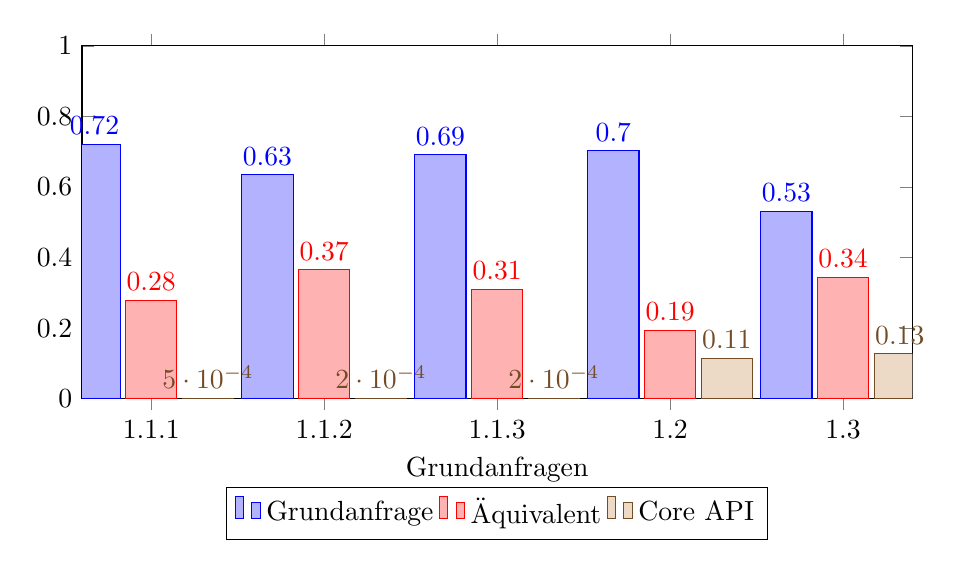
\begin{tikzpicture}
\centering
  \begin{axis}[
ybar,
bar width=.65cm,
width=\textwidth,
height=.5\textwidth,
legend style={at={(0.5,-0.25)},
	anchor=north,legend columns=-1},
symbolic x coords={1.1.1,1.1.2,1.1.3,1.2,1.3},
xtick=data,
nodes near coords,
nodes near coords align={vertical},
ymin=0,ymax=1,
xlabel={Grundanfragen},
]

\addplot coordinates {(1.1.2,0.6345) (1.1.1,0.7211)(1.1.3,0.6908)(1.2,0.7025) (1.3,0.5297)};
\addplot coordinates {(1.1.2,0.3652) (1.1.1,0.2783)(1.1.3,0.3089)(1.2,0.1935) (1.3,0.3434)};
\addplot coordinates{(1.1.2,0.0002)(1.1.1,0.0005)(1.1.3,0.0002)(1.2,0.1139)(1.3,0.1269)};
\legend{Grundanfrage,Äquivalent,Core API}
\end{axis}
\end{tikzpicture}
\captionof{figure}{Übersicht der Anfragen aus dem ersten Testlauf} 
\label{ref:Compare1}
\end{center}
\FloatBarrier

\subsection{Ergebnisse des zweiten Testlaufes}
In der Grundanfrage 2.1.1
\begin{Verbatim}[frame=single]
MATCH(p:Person{name:'Person1'})-[:RELATIONSHIP3*2]->(p1:Person) 
RETURN COUNT(DISTINCT(p1))
\end{Verbatim}
 wurden bei der Traversierung bis zur Tiefe 2 ausgehend von Person1 99 \% aller Knoten des Graphen erreicht. Bei der Tiefe3 wurden alle Knoten erreicht. Wie Tabelle \ref{tab:Query2_1} zeigt, besteht zwischen der Traversierung bis zur Tiefe 2 und Tiefe 3  ein minimaler zeitlicher Unterschied von durchschnittlich ca. 5,6\%, dies widerspricht der Hypothese, dass die Zeit in Cypher doppelt so hoch sein wird. Es besteht so kein direkter Zusammenhang zwischen der Anzahl der zu betrachtenden Knoten und der Bearbeitungszeit. Wie erwartet verändert sich die Berechnungszeit nur minimal bei der Breiten- und Tiefensuche, wenn die Tiefe um 1 erhöht wird.  \newline 
Es wurde bestätigt, dass die Anfrage mit Tiefensuche signifikant schneller als die Anfrage mit Breitensuche ausgeführt wird, in diesem Fall ist die Anfrage für die Tiefe 2 ca. 60\% schneller. Dies wurde in Kapitel 3 durch das Verhältnis der Breite zur Tiefe begründet. 
\FloatBarrier
\begin{table}[h]
\centering
		\begin{tabular}{ |p{3cm}||p{3cm}|p{3cm}|p{3cm}|  }
			\hline
			Anfrage& Cypher & Breitensuche&Tiefensuche\\
			\hline
			Tiefe 2   & 224431    & 5101&  2076\\
			Tiefe 3&    234132  & 1278   & 89\\
			\hline
		\end{tabular}
		\caption{Grundanfragen 2.1.1 und 2.1.2}
		\label{tab:Query2_1}
\end{table}
\FloatBarrier
\noindent Wie Tabelle \ref{tab:Query2_2} zeigt, besteht kein  signifikanter Unterschied zwischen Grundanfrage 2.2
\begin{Verbatim}[frame=single]
MATCH t=(p:Person{name :'Person1'})-[:RELATIONSHIP3]->(p1:Person)
-[:RELATIONSHIP3]->(p2)
WHERE NOT (p)-[:RELATIONSHIP3]->(p2) 
RETURN COUNT(DISTINCT(p2))
\end{Verbatim} 
 und der äquivalenten Anfrage in Cypher. Beide Anfragen sind um ein vielfaches langsamer als die Anfrage, die die Core API verwendet. In der Core API Anfrage wurden 2 Ergebnismengen vom Java-typ $Set$ gebildet und durch den Aufruf der Funktion $removeAll()$  wurden die Elementen der einen Mengen aus der anderen Menge entfernt. Dies entspricht einer Realisierung von dem $Where\;not$ Ausdruck  in Java und besitzt eine bessere Performanz. Alle 3 Anfragen besitzen im Vergleich zu vorangegangen Anfragen eine extrem hohen Ausführungszeit.
\FloatBarrier
\begin{table}[h]
	\centering
		\begin{tabular}{ |p{3cm}|p{3cm}|p{3cm}|p{3cm}|  }
			\hline
			Grundanfrage 2.2 & Äquivalent&Core API\\
			\hline
			4740646    & 4753414 &  1609\\
			\hline
		\end{tabular}
		\caption{Grundanfrage 2.2}
		\label{tab:Query2_2}
\end{table}
\FloatBarrier
\noindent Der kürzeste Pfade, welcher in Grundanfrage 2.3
\begin{Verbatim}[frame=single]
MATCH (p:Person{name :'Person1'}),(p1:Person{name :'Person42'}),
path=shortestPath((p)-[:RELATIONSHIP4*..3]->(p1)) 
RETURN LENGTH(path)
\end{Verbatim} 
 untersucht wurde, besitzt die Länge 2. Die Grundanfrage 2.1.1 zeigt, dass bei einer Pfadlänge von 2 die meisten Knoten ausgehend von Person1 erreicht werden. Wie in Tabelle \ref{tab:Query2_3} zu sehen, ist die Ausführungszeit der Anfrage in Cypher unter Verwendung des gegebenen Algorithmus, geringer als alle anderen Grundanfragen außer Grundanfrage 1.2. Erstmalig ist die Anfrage in Cypher schneller als die alternative Formulierung in der Core API. Der relative Unterschied beträgt 37 \% und  der absolute Unterschied 3,1 ms. Durch die geringe absolute Differenz ist es nicht garantiert, dass der kürzeste Pfad mit der Verwendung von Cypher immer die schnellste Schnittstelle darstellt. \newline
Die äquivalente Formulierung in Cypher besitzt die höchste aller beobachtetet Ausführungszeiten mit ca. 2,3 Stunden. Diese Formulierung ist eine naiver Ansatz ohne Verwendung des Algorithmus und besitzt viele Berechnungsschritten, die durch den Algorithmus entfallen würden. Zudem stoppt der Limit-Ausdruck nicht vorzeitig die Berechnung, sondern filtert die Ergebnismenge erst nach der Berechnung, dieses Verhalten ist mit der konservativen Stop-Strategie aus SQL zu vergleichen\parencite{carey1997saying}.   
\FloatBarrier
\begin{table}[!htb]
	\centering
		\begin{tabular}{ |p{3cm}|p{3cm}|p{3cm}|p{3cm}|  }
			\hline
			Grundanfrage 2.3 & Äquivalent&Core API\\
			\hline
			8,4    & 8370298 &  11,5\\
			\hline
		\end{tabular}
		\caption{Grundanfrage 2.3}
		\label{tab:Query2_3}
\end{table}
\FloatBarrier
\noindent Die Ergebnisse der Traversierungen des gesamten Graphen, wie in Grundanfrage 2.4
 \begin{Verbatim}[frame=single]
MATCH (a)-[RELATIONSHIP4]->(b) RETURN COUNT(DISTINCT(b))
\end{Verbatim}
 werden in Tabelle \ref{tab:Query2_4} dargestellt.
 In der Core API ist die einseitige Traversierung mit Breitensuche ca. 4,8\% langsamer als der gleiche Algorithmus bei einer bidirektionalen Traversierung. Bei der Tiefensuche beträgt der Unterschied ca. 13\%. In beiden Fällen sind die einseitigen Traversierungen wie erwartet langsamer als die bidirektionale Alternativen. \newline
Trotz einer semantischen Äquivalenz von Grundanfrage 2.4.1 mit der Grundanfrage 2.1.2, bei der alle Knoten erreicht werden, ist eine signifikant höhere Ausführungszeit zu beobachten. Dieses Verhalten lässt sich nur mit dem Fehlen einer frühzeitigen Abbruchbedingung erklären.    
\FloatBarrier
\begin{table}[!htb]
	\centering
	\begin{tabular}{ |p{5cm}||p{3cm}|p{3cm}|p{3cm}|  }
		\hline
		Anfrage & Zeit\\
		\hline
		Grundanfrage 2.4.1 & 284594\\
		\hline
		Vergleichsanfrage 1 & 31020  \\
		\hline
		Grundanfrage 2.4.2 & 31050\\
		\hline
		Grundanfrage 2.4.3 &  29558  \\
		\hline
		Grundanfrage 2.4.4 &  26982\\
		\hline
	\end{tabular}
	\caption{Grundanfragen 2.4.1-2.4.4}
	\label{tab:Query2_4}
\end{table}
\FloatBarrier

\subsection{Ergebnisse des dritten Testlaufes}
Für die folgenden Aussagen werden die Werte aus der Tabelle \ref{tab:Query3}  betrachtet. Dieses Tabelle stellt die Zeiten der Grundanfragen, ihrer Äquivalente in der Core API und in der OrientDB dar. \newline
Die Grundanfragen 1.1.1-1.1.3 werden in Cypher durchschnittlich ca. 12 mal schneller ausgeführt als in der OrientDB, die relativ langen Bearbeitungszeiten bei beiden Systemen entstehen durch die Bedingungen im Where-Prädikat. In allen Fällen benötigt die Grundanfrage 1.1.3, welche die eingehenden und ausgehenden Kanten betrachtet, die längste Zeit zur Bearbeitung. Im Vergleich zu Neo4j und den anderen Anfragen, die an OrientDB gestellt wurden, benötigen die Grundanfragen 1.1.1-1.1.3 in OrientDB extrem viel Zeit zur Bearbeitung. Dies zeigt, dass OrientDB wie Neo4j durch das Einfügen einer Bedingung im Where-Prädikat sehr stark beeinflusst wird und bei solchen Anfragen eine langsame Berechnung ausführt. \newline
 Grundanfrage 1.2, welche solange über den Graphen traversiert bis ein bestimmter Knoten gefunden ist, weist in OrientDB eine schnellere Bearbeitungszeit als Neo4j mit der Core API oder Cypher auf und wird ca. 3,7 mal schneller bearbeitet als die in Cypher gestellte Anfrage. Die Grundanfragen 2.1.1 und 2.1.2, welche ebenfalls mit einer Abbruchbedingung über den Graphen traversieren, werden auf OrientDB ca. 2,6 mal schneller ausgeführt als auf Neo4j mit Cypher. Daraus lässt sich schließen, dass OrientDB  bei einer Traversierung mit frühzeitigem Abbruch eine bessere Performanz besitzt als Neo4j unter der Verwendung von Cypher. Bei einer kompletten Traversierung des Graphen wie in den Grundanfrage 2.4.1 und 2.4.2, besitzt Neo4j mit der Core API oder mit Cypher eine bessere Performanz als OrientDB. In Cypher wird die Grundanfrage 2.4.1 ca. 2,7 mal schneller bearbeitet als die gleiche Anfrage in SQL mit OrientDB und mit der Core API wird die Anfrage ca. 27 mal schneller beantwortet. \newline
Grundanfrage 1.3, welche eine einfache Anfrage zum Finden von gemeinsamen Nachbarn darstellt, besitzt in Cypher und der Core API eine relativ geringe Bearbeitungszeit in der Größenordnung von einigen Millisekunden. In OrientDB befindet sich Grundanfrage 1.3 mit einer benötigten Zeit von 83955 ms in einer anderen Größenordnung und deutet darauf hin, dass der Vergleich von 2 Mengen miteinander in Neo4j effizienter implementiert ist. Dies ist auch in Grundanfrage 2.2 zu beobachten, für diese Anfrage muss bis in die Tiefe 2 traversiert werden und 2 Mengen müssen miteinander verglichen werden. Die Anfrage besitzt eine extrem hohe Bearbeitungszeit, obwohl das Traversieren in der Tiefe 2, wie bei Grundanfrage 2.1.1 mit 72092 ms zu beobachten, eine relative geringe Zeit benötigt, der Vergleich der beiden Mengen bildet so den rechenaufwendigeren Schritt. \newline
 Wie bei Core API von Neo4j besteht ein Unterschied von ca. 35 \% zwischen den Grundanfragen 2.1.1 und 2.1.2, obwohl die Anzahl der zu betrachtenden  Knoten um den Faktor 2500 ansteigt. Dies deutet auf eine sehr gute Skalierbarkeit bei beiden Systemen hin, da bei beiden Systemen die Bearbeitungszeiten in einer weniger als linearen Faktor zu den betrachtenden Knoten ansteigt. \newline  
 Grundanfrage 2.2 konnte in dieser Evaluation nicht vollständig analysiert werden, da die erste Ausführung der Anfrage ohne Caching ungefähr 70 Stunden benötigt hat. Weitere Wiederholungen mit Caching waren nicht möglich, aber benötigen mit hoher Wahrscheinlichkeit auch mehrere Stunden bzw. Tage. \newline
Mit 37,6 ms benötigt OrientDB bei Grundanfrage 2.3 ähnlich wie Neo4j eine relativ kurze Bearbeitungszeit, dies lässt sich durch eine effiziente Implementierung des shortestpath-Algorithmus erklären. Da das Finden des kürzesten Pfades eine grundlegendes Problem bei Graphen ist, wurde der Algorithmus bereits in der OrientDB Version 1.7.8 vom 13. August 2014 veröffentlicht\footnote{https://orientdb.com/released-orientdb-1-7-8/}. Durch die frühe Zurverfügungstellung ist es wahrscheinlich, dass der Algorithmus mit einer effizienten Implementierung veröffentlicht wurde oder über die Jahre optimiert wurde. \newline
Für die Grundanfrage 2.4.2, welche mit Breitensuche über den gesamte Graphen traversiert, ist nur ein Vergleich zwischen OrientDB und der Core API von Neo4j möglich, da der Such-Algorithmus in Cypher nicht explizit angegeben werden kann und immer Tiefensuche verwendet wird. Durch die gleiche Komplexität von O(V+E) bei der Tiefen- und Breitensuche, benötigen die Grundanfragen 2.4.1 und 2.4.2 in OrientDB ungefähr die gleiche Bearbeitungszeit. In Cypher wird die Grundanfrage 2.4.1 ca. 2,7 mal schneller bearbeitet. Mit Verwendung der Core API wird die einseitige Tiefen- und Breitensuche durchschnittlich ca. 24.8 mal schneller beantwortet als auf OrientDB. Dabei muss berücksichtigt werden, dass die Core API ein hohes technisches Verständnis voraussetzt und nahe an den Kernfunktionen arbeitet und OrientDB die Anfragesprache SQL verwendet, welche eine weniger abstrakte Schnittstelle für den Nutzer darstellt und durch den Abstand zum Kern eine geringere Performanz besitzt. \newline
Insgesamt besitzt die Core API von Neo4j in fast allen Fällen eine signifikant bessere Performanz als OrientDB. Der direkte Vergleich zwischen den Anfragesprachen der beiden Systeme zeigt, dass OrientDB in einigen Fällen, wie dem nicht-vollständigen Traversieren des Graphen, eine bessere Performanz aufweist. Unter der Berücksichtigung aller beobachteten Zeiten besitzen beide Anfragesprachen Stärken und Schwächen, wodurch sich keine allgemeine Aussage über eine bessere Performanz von einer der beiden Sprachen treffen lässt. 
\FloatBarrier
\begin{table}[h]
	\centering
	\begin{tabular}{ |p{6cm}||p{2cm}|p{2cm}|p{2cm}|  }
		\hline
		Anfrage& Cypher & OrientDB & Core API \\
		\hline
	Grundanfrage 1.1.1  & 215383 & 3495459    &  64\\
	Grundanfrage 1.1.2& 212620 & 1674758   & 160   \\
	Grundanfrage 1.1.3& 496704 & 6350806 & 165  \\
	Grundanfrage 1.2& 0,54 & 0,17   & 0,29   \\
	Grundanfrage 1.3 & 8,66& 83955  & 3,2    \\
	Grundanfrage 2.1.1& 224431 & 72092   & 2076   \\
	Grundanfrage 2.1.2& 234132& 110064  & 89    \\
	Grundanfrage 2.2& 4740646 &  $\approx$ 70h   & 1609  \\
	Grundanfrage 2.3& 8,4  & 37,6   & 11,5   \\
	Grundanfrage 2.4.1& 284594 & 768830  & 31050\\
	Grundanfrage 2.4.2& -  & 774040   & 31020   \\
		\hline
	\end{tabular}
	\caption{Grundanfragen auf Neo4j und OrientDB}
	\label{tab:Query3}
\end{table}
\FloatBarrier
\section{Anwendungsszenario}
Neoj4 Inc. stellt zahlreiche Nutzungen von Graphen in verschiedenen Themenkomplexen vor\footnote{https://neo4j.com/graphgists/ (10.09.18)}. Für jeden Themenkomplex werden mehrere Beispielgraphen von eigenständigen Entwicklern, welche nicht für Neo4j arbeiten, zur Verfügung gestellt. Das folgende Anwendungsszenario stellt den Zweck einer Graphdatenbank für Kinofilme dar.\newline
In diesem Beispiel ist der Nutzer ein Betreiber eines Kinos, welches aktuelle Kinofilm ausstrahlt und besondere Veranstaltungen betreibt. Bei diesen Veranstaltungen werden mehrere Filme von einer Kategorie oder einem bestimmten Schauspieler oder Regisseur gezeigt. Diese Veranstaltungen werden mehrere Wochen vor dem Veranstaltungstermin verplant und finden über mehrere Tage statt. Pro Veranstaltungstag werden im Durchschnitt 4 Filme benötigt. Solche Veranstaltungen wurden schon mehrmals betrieben und die Planung besitzt einen routinierten Ablauf, sodass viele Schritte effizient bearbeitet werden. Der zeitaufwendigste Arbeitsschritt, stellt das Finden von Filmen für das Veranstaltungsprogramm dar. \newline
Aktuell stellt der Kinobetreiber eine Liste mit Filmen für die Veranstaltung manuell zusammen, hierfür werden Filme ausgewählt, die der Betreiber selber kennt und es werden verschiedene Quellen aus dem Internet für eine Auswahl verwendet. Die Liste besitzt die Namen der Filme, zusätzliche Informationen wie Länge sind durch die Vielzahl von Quellen nicht immer vorhanden. Fehlende Informationen müssen für eine optimale Planung des Kinoprogramms erneut herausgesucht werden und einige Filme müssen nach dem initialen Aufstellen der Liste  aussortiert werden. \newline  
Für eine Beschleunigung dieses Arbeitsschrittes kann das Datenbankmanagementsystem Neo4j verwendet werden. Unabhängig von dem Betriebssystem steht die kostenfreie Anwendung $Neo4j\; Desktop$ zur Verfügung. Durch diese Anwendung für den Desktop ist die Bedienung von Neo4j über ein grafischen User Interface(GUI) möglich. Zusätzlich wird die Erweiterung $APOC$ benötigt, welche per Mausklick in $Neo4j\; Dekstop$ eingebunden werden kann. Mit dieser Erweiterung ist es möglich Daten mit verschiedenen Dateiformaten wie CSV in die lokale Neo4j Datenbank zu importieren. Für das Thema Kino stehen im Internet zahlreiche große Datensätze mit Filme kostenfrei zur Verfügung \footnote{https://www.kaggle.com/carolzhangdc/imdb-5000-movie-dataset}. Nach dem Importieren eines solchen Datensatzes, kann der Nutzer durch die Eingabemaske eine Anfrage stellen, um so eine übersichtliche vollständige Liste von Filme zu erhalten. Eine beispielhafte Anfrage in Cypher für eine Liste von Verbrechen-Filmen ist: 
\begin{Verbatim}[frame=single]
MATCH(m:Film) 
WHERE m.Katergorie = Verbrechen
RETURN m.Name as Name, m.Regie as Regie, 
	m.Länge as Länge, m.Plot as Plot 
LIMIT 20
\end{Verbatim}
Diese Anfrage erstellt eine Liste von 20 Filme, die für eine Veranstaltung mit Verbrechen-Filmen passen. Weitere Bedingungen können durch die Cypher Syntax einfach eingefügt werden, beispielsweise wenn gut bewertete Filme von einem Schauspieler gesucht werden:
\begin{Verbatim}[frame=single]
MATCH(s:Schauspieler)-[SpielteIn]->(f:Film) 
WHERE s.Name = 'Peter Dinklage' AND f.Wertung >= 5
RETURN f.Name as Name, f.Regie as Regie, 
	f.Länge as Länge, f.Plot as Plot 
LIMIT 20
\end{Verbatim}
Neo4j übernimmt so das Auswerten von einem Datensatz, der beispielsweise in einem CSV Format dargestellt wird und für den Nutzer schwer zu lesen ist. Durch die effiziente Implementierung von Neo4j wird in kurzer Zeit eine vollständige Liste mit Filmen erstellt, die geforderte Bedingungen erfüllen. Der Arbeitsschritt zum Erstellen einer Liste mit geeigneten Filmen wird damit stark beschleunigt und effizienter ausgeführt.
\section{Limitierungen und zukünftige Arbeit}
Die durchgeführte Evaluation nutzt mit OrientDB  eine einzige Referenzdatenbank. Dies ist keine reine GDB und unterstützt weitere Typen von Datenbanken. Für eine näherer Einordnung der Performanz von Neoj4 ist ein Vergleich mit einer reinen GDB wie beispielsweise der Sparksee Database sinnvoll\footnote{http://www.sparsity-technologies.com/ (28.08.19)}. Diese Datenbank konnte in dieser Evaluation auf Grund von Kommunikationsprobleme mit Sparsity technologies nicht verwendet werden. Durch einen Vergleich mit der Sparksee Database könnte die Performanz von zahlreichen Graphalgorithmen   wie zum Beispiel Zentralitäts-Algorithmen überprüft werden. Dies ist mit OrientDB nicht direkt möglich, da keine vergleichbare Implementierung der von Neo4j unterstützen Graphalgorithmen im vollen Ausmaß in OrientDB gegeben ist. \newline 
Ein Vergleich zwischen Neo4j und einer relationalen Datenbank, wie in \parencite{vicknair2010comparison} beschrieben, ist für eine weitere Beschreibung der Vor- und Nachteile einer Graphdatenbank sinnvoll. Dieser Vergleich wurde aus zeitlichen Gründen nicht vollzogen. Die Referenz zur OrientDB hat einen Vergleich zu einer anderen noSQL-Datenbank dargestellt und so ein erste Einschätzung zu der Performanz von Neo4j ermöglicht. \newline
Ein weitere Aspekt der betrachtet werden kann, ist das Ausführen von Neo4j im Server Modus und auf mehreren Geräten verteilt. Durch diesen Aspekt können die ACID und CAP Eigenschaften genau untersucht werden und die Grenzen einer verteilten Neo4j-Datenbank getestet werden. Zudem kann ein Vergleich zwischen der Datenbank im eingebetteten Modus und dem Server Modus durchgeführt werden. So können genaue Vor- und Nachteile und ein Anwendungsszenario spezifiziert werden. \newline
Eine kleinerer nicht betrachteter Aspekt ist die temporale Eigenschaft von Neo4j. Der vorgestellte Datensatz besitzt Attribut vom Typen $Date$ und stellt so eine temporale Datenbank dar, doch es fehlt ein Testlauf mit Anfragen zu diesem Attribute. Eine Allgemeine Betrachtung des temporalen Verhalten der Datenbank ist für eine genauere Einordnung von Neo4j im Vergleich zu anderen temporalen Graphdatenbanken sinnvoll. 
\section{Fazit}
Neo4j unterstützt mit den Java-Standardtypen und zahlreichen zeitlichen Typen wie $Time$, $LocalTime$ oder $DateTime$ eine Vielzahl von Datentypen, welche für die Modellierungen von Daten notwendig sind\footnote{https://neo4j.com/docs/cypher-manual/current/syntax/values/ (28.08.19)}. Durch die Zurverfügungstellung der Anwendungen $Neo4j\; Dekstop$ und $Neo4j\; Browser$ und einer dazu gegebenen Anfragesprache, werden die benötigten Kenntnisse zur Bedienung des System minimiert. Für eine spezifischeren Gebrauch der Datenbank, werden mehrere Programmiersprachen unterstützt. Durch diese Schnittstellen ist es mögliche, das System auf viele Weisen zu nutzen und eine große Zielgruppe kann das System für viele Szenarien verwenden. \newline 
Testlauf 1 und 2 zeigen, dass der Gebrauch der Java Core API in allen Fällen zu einer signifikant besseren Performanz führt. Mit Verwendung der Traversal API besitzt der Nutzer eine flexible Möglichkeit die Performanz seiner Anfragen zu beeinflussen. Zum Beispiel ist es möglich zwischen Breiten- und Tiefensuche zu wählen. Die am schnellsten bearbeiteten Anfragen besitzen keine gemeinsame Kategorie von den vorgestellten Kategorien aus Absatz \ref{Kategorien}. Die am langsamsten bearbeiteten Anfragen besitzen ebenfalls keine gemeinsamen Kategorien. Grundanfrage 2.2, welche die einzige Mustervergleichs-Anfrage ist, besitzt eine besonders hohe Ausführungszeit. Dementsprechend lässt sich nur für Mustervergleichs-Anfragen ein Bezug von Anfragen-Kategorie und Performanz in Neo4j erkennen, die anderen Kategorien weisen keinen solchen Bezug auf. \newline
Wie die Tabellen \ref{tab:Query1_2} und \ref{tab:Query2_3} zeigen, können semantisch gleiche Anfragen in Cypher Unterschiede in ihrer Performanz aufzeigen. Dieses Verhalten ist in den APIs ebenfalls zu beobachten. Das System lässt sich durch eine hohe Anzahl von Schnittstellen leicht benutzten, aber das System effektiv zu nutzen und eine Anfrage effizient ausführen zu lassen, ist nicht trivial und erfordert technologische Kenntnisse. Durch Hinweise von Neo4j Inc. werden einige Möglichkeiten für das effiziente Ausführen gegeben \footnote{https://neo4j.com/blog/tuning-cypher-queries/ (07.08.19)}. Diese Hinweise befassen sich teilweise mit dem Umformulieren der Anfragen, um das volle Potenzial des Optimierers nutzen zu können. Wie in den Ergebnissen zur Grundanfrage 1.2 erläutert, deutet dies unter anderem auf einen unperformanten Optimierer hin. \newline
Im Vergleich zu der Muli-Model Datenbank OrientDB unter Verwendung von SQL besitzt Neo4j mit der Core API ein signifikant bessere Performanz. Mit  Anfragesprache Cypher ist die Performanz von Neo4j nicht mehr eindeutig besser. Der verwendete Datensatz ist unter Neo4j ca. 58 \% größer, als bei OrientDB. Allgemein besitzt Neo4j so eine bessere Performanz, wenn die Kenntnisse durch den Nutzer gegeben sind, aber die Speicherverwaltung unter Neo4j ist schlechter. Wie die Performanz im globalen Kontext im Vergleich zu mehreren anderen Datenbankmanagementsystemen ist, wie in \parencite{jouili2013empirical} ausgeführt,  lässt im Rahmen dieses Experiments nicht sagen. 

\begin{acknowledgements}
	An dieser Stelle möchte ich all jenen danken, die durch ihre fachliche und persönliche Unterstützung zum Gelingen dieser Bachelorarbeit beigetragen haben. \newline \newline
	Ebenso gilt mein Dank Melf und Lasse für das Korrekturlesen. Zuletzt möchte ich noch all denjenigen danken, die in der Zeit der Erstellung dieser Arbeit für mich da waren, insbesondere meinen Freunden. \newline \newline
	Schließlich danke ich meinen Freunden während der Studienzeit für drei sehr schöne Jahre in Lübeck.
\end{acknowledgements}